\documentclass[aspectratio=169]{beamer}
\usepackage{hyperref}
\usepackage{listings}
\usepackage{tkz-berge}
\setbeamertemplate{caption}[numbered]

% \usepackage{fontspec}
% \setmonofont{Consolas}

\definecolor{background}{RGB}{39, 40, 34}
\definecolor{string}{RGB}{230, 219, 116}
\definecolor{comment}{RGB}{117, 113, 94}
\definecolor{normal}{RGB}{248, 248, 242}
\definecolor{identifier}{RGB}{166, 226, 46}
\definecolor{keyword}{HTML}{F92672}
\definecolor{numbers}{HTML}{AE81FF}
\definecolor{types}{HTML}{66D9EF}


\lstset{
    language=C++,
    tabsize=4, % tab space width
    showstringspaces=false, % don't mark spaces in strings
    numbers=left, % display line numbers on the left
    basicstyle=\ttfamily,
    numberstyle=\color{comment}\ttfamily, % Line numbers
    commentstyle=\color{comment}\ttfamily, % comment color
    otherkeywords={>,<,-,!,=,~}, % Color operators too
    morekeywords={>,<,-,!,=,~},
    keywordstyle=\color{keyword}\ttfamily, % keyword color
    stringstyle=\color{string}\ttfamily, % string color
    morecomment=[l][\color{keyword}]{\#},
    emph={int,char,long,float,double,unsigned,namespace,typename},
    emphstyle={\color{types}\ttfamily\textit},
    escapeinside={@!}{!@},
    captionpos=b
}
\newcommand{\code}{\texttt}
\newcommand{\fn}{\color{identifier}}
\renewcommand*{\thefootnote}{\fnsymbol{footnote}}
\usetheme{Warsaw}

\addtobeamertemplate{footnote}{\vspace{-6pt}\advance\hsize-0.5cm}{\vspace{6pt}}
\makeatletter
% Alternative A: footnote rule
\renewcommand*{\footnoterule}{\kern -3pt \hrule \@width 2in \kern 8.6pt}
% Alternative B: no footnote rule
% \renewcommand*{\footnoterule}{\kern 6pt}
\makeatother

\setbeamercolor{normal text}{fg=normal,bg=background}
\setbeamercolor{structure}{fg=normal}

\setbeamercolor{alerted text}{fg=red!85!black}

\setbeamercolor{item projected}{use=item,fg=background,bg=item.fg!35}

\setbeamercolor*{palette primary}{use=structure,fg=structure.fg}
\setbeamercolor*{palette secondary}{use=structure,fg=structure.fg!95!black}
\setbeamercolor*{palette tertiary}{use=structure,fg=structure.fg!90!black}
\setbeamercolor*{palette quaternary}{use=structure,fg=structure.fg!95!black,bg=black!80}

\setbeamercolor*{framesubtitle}{fg=normal}

\setbeamercolor*{block title}{parent=structure,bg=background}
\setbeamercolor*{block body}{fg=black,bg=background}
\setbeamercolor*{block title alerted}{parent=alerted text,bg=background}
\setbeamercolor*{block title example}{parent=example text,bg=background}

\title{Interview Skills}
\subtitle{Graph Algorithms}
\author{Richard Morrill}
\institute{Fordham University CS Society}
\logo{
\includegraphics[width=2cm]{css_logo_color.png}}
\date{Wednesday, January 9th 2019}

\section{}
\begin{document}
\begin{frame}
\titlepage
\end{frame}


\begin{frame}
    \frametitle{What is a Graph?}
    \pause
    \begin{figure}
    \begin{minipage}[c]{0.4\textwidth}
            \centering
            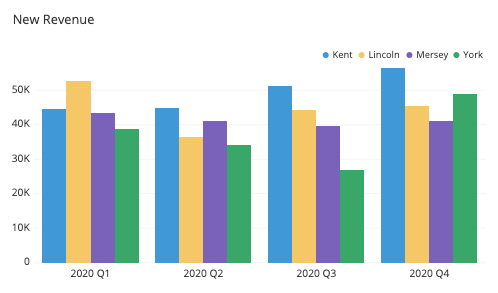
\includegraphics{bar_chart_example.png}
            \caption{Not This Kind of Graph!}
            \label{bargraph}
    \end{minipage}
    \hfill
    \pause
    \begin{minipage}[c]{0.4\textwidth}
            \centering
            \begin{tikzpicture}[draw=white,color=white]

                \tikzset{vertex/.style = {shape=circle,draw,minimum size=1.5em}}
                \tikzset{edge/.style = {->,> = latex'}}
                \node[vertex] (a1) at (0,0) {a1};
                \node[vertex] (a2) at (0,2) {a2};
                \node[vertex] (a3) at (2,0) {a3};
                \node[vertex] (a4) at (2,2) {a4};

                \draw[edge] (a1) to (a2);
                \draw[edge] (a1) to[bend left] (a4);
                \draw[edge] (a4) to[bend left] (a1);
                \draw[edge] (a2) to (a3);

            \end{tikzpicture}
            \caption{This Kind of Graph!}
            \label{fullyconnectedex}
        \end{minipage}
    \end{figure}
\end{frame}
\begin{frame}
    \frametitle{Characteristics of a Graph}
    \begin{itemize}
        \item Set of Nodes $S$
        \item Set of Edges $E \subset S^{2}$\footnote[frame]{This just means every possible ordered pair of nodes.}
        \pause
        \item Can represent a wide variety of real-world problems (such as?)
        \pause
        \begin{itemize}
            \item Islands \& Bridges
            \item Network Connections\only<3->\footnote[frame]{You'll see this come up when you take a networking class.}
            \item Intersections and Streets
        \end{itemize}
        \pause
        \item Position of nodes is for communication only
        \item Edges may have a ``weight'' assigned to them, which may represent distance in some cases
    \end{itemize}
\end{frame}
\begin{frame}
    \frametitle{Adjacency Matrix}
    \begin{itemize}
        \item Very useful for mathematical proofs
        \begin{figure}
            \begin{minipage}[c]{0.4\textwidth}
                \centering
                \begin{tikzpicture}[draw=white,color=white]

                    \tikzset{vertex/.style = {shape=circle,draw,minimum size=1.5em}}
                    \tikzset{edge/.style = {->,> = latex'}}
                    \node[vertex] (a1) at (0,0) {a1};
                    \node[vertex] (a2) at (0,2) {a2};
                    \node[vertex] (a3) at (2,0) {a3};
                    \node[vertex] (a4) at (2,2) {a4};
    
                    \draw[edge] (a1) to (a2);
                    \draw[edge] (a1) to[bend left] (a4);
                    \draw[edge] (a4) to[bend left] (a1);
                    \draw[edge] (a2) to (a3);
                    \draw[edge] (a1) to [loop below] (a1);
    
                \end{tikzpicture}
                \caption{Visual Representation of a Graph}
                \label{visgrap}
            \end{minipage}
            \hfill
            \begin{minipage}[c]{0.4\textwidth}
                \centering
                $\begin{pmatrix}
                    1 & 1 & 0 & 1 \\
                    0 & 1 & 0 & 0 \\
                    0 & 0 & 0 & 0 \\
                    1 & 0 & 0 & 0
                \end{pmatrix}$
                \caption{The Same Graph as \ref{visgrap}, in an Adjacency Matrix}
                \label{}
            \end{minipage}
        \end{figure}
        \pause
        \item Memory usage causes issues when used in programs.
    \end{itemize}
\end{frame}
\begin{frame}
    \frametitle{Representations of Graphs in Code}
    \begin{itemize}
        \item A graph is an \textbf{abstract data type (ADT)}
        \pause
        \begin{itemize}
            \item The operations you can perform on a graph are consistently defined.
            \item The actual way data is stored may vary from implementation to implementation.
        \end{itemize}
        \pause
        \item For higher level problems, you might use a graph library that provides a consistent interface to access and manipulate graphs.
        \item For now, though, it's important to show you know how to actually work with low-level implementations.
        \pause
        \item Graphs are most often represented as:
        \begin{itemize}
            \item Node Lists
            \item Edge Lists
        \end{itemize}
    \end{itemize}
\end{frame}
\begin{frame}[fragile]
    \frametitle{Node List}
    \begin{columns}
        \begin{column}{0.5\textwidth}
            \begin{tikzpicture}[draw=white,color=white]

                \tikzset{vertex/.style = {shape=circle,draw,minimum size=1.5em}}
                \tikzset{edge/.style = {->,> = latex'}}
                \node[vertex] (0) at (0, 4) {0};
                \node[vertex] (1) at (3, 4) {1};
                \node[vertex] (2) at (0, 2) {2};
                \node[vertex] (3) at (3, 2) {3};
                \node[vertex] (4) at (1.5, 0) {4};

                \draw[edge] (0) to [loop above] (0);
                \draw[edge] (0) to (4);

                \draw[edge] (1) to (2);
                \draw[edge] (1) to [bend right] (3);
                \draw[edge] (1) to (0);

                \draw[edge] (2) to (0);
                \draw[edge] (2) to (4);

                \draw[edge] (3) to [loop right] (3);
                \draw[edge] (3) to [bend right] (1);
                \draw[edge] (3) to [bend right] (4);

                \draw[edge] (4) to [bend right] (3);
            \end{tikzpicture}
        \end{column}
        \begin{column}{0.5\textwidth}
            \begin{lstlisting}
vector<vector<int>> graph = {
    {0, 4},
    {2, 3, 0},
    {0, 4},
    {3, 1, 4},
    {3}
};
            \end{lstlisting}
        \end{column}
    \end{columns}
\end{frame}
\begin{frame}[fragile]
    \frametitle{Edge List}
    \begin{columns}
        \begin{column}{0.5\textwidth}
            \begin{tikzpicture}[draw=white,color=white]

                \tikzset{vertex/.style = {shape=circle,draw,minimum size=1.5em}}
                \tikzset{edge/.style = {->,> = latex'}}
                \node[vertex] (0) at (0, 4) {0};
                \node[vertex] (1) at (3, 4) {1};
                \node[vertex] (2) at (0, 2) {2};
                \node[vertex] (3) at (3, 2) {3};
                \node[vertex] (4) at (1.5, 0) {4};

                \draw[edge] (0) to [loop above] (0);
                \draw[edge] (0) to (4);

                \draw[edge] (1) to (2);
                \draw[edge] (1) to [bend right] (3);
                \draw[edge] (1) to (0);

                \draw[edge] (2) to (0);
                \draw[edge] (2) to (4);

                \draw[edge] (3) to [loop right] (3);
                \draw[edge] (3) to [bend right] (1);
                \draw[edge] (3) to [bend right] (4);

                \draw[edge] (4) to [bend right] (3);
            \end{tikzpicture}
        \end{column}
        \begin{column}{0.5\textwidth}
            \begin{lstlisting}
vector<vector<int>> graph = {
    {0, 0},
    {0, 4},
    {1, 2},
    {1, 3},
    {1, 0},
    {2, 0},
    {2, 4},
    {3, 3},
    {3, 1},
    {3, 4},
    {4, 3}
};
            \end{lstlisting}
        \end{column}
    \end{columns}
\end{frame}
\begin{frame}
    \frametitle{Graph Operations}
    \begin{itemize}
        \item Part of the graph ADT
        \item Theoretical functions you can perform on nodes
        \pause
        \item View Operations
        \begin{itemize}
            \item adjacent(x,y): bool
            \item neighbors(x): list of edges
            \item get\_vertex\_value(x): value type
            \item get\_edge\_value(\dots): value type\only<2->\footnote[frame]{Argument is either edge key or the two vertices it connects, depending on representation.}
        \end{itemize}
        \pause
        \item Modify Operations\only<3->\footnote[frame]{We won't be modifying already constructed graphs in this workshop.}
        \begin{itemize}
            \item set\_vertex\_value(x, v): void
            \item set\_edge\_value(\dots, v): void
            \item add / remove edges / vertices
        \end{itemize}
    \end{itemize}
\end{frame}
\begin{frame}
    \frametitle{Properties of a Graph}
    \begin{itemize}
        \item This is information you might be given as part of an interview prompt.
        \item If you misinterpret it, you're basically guaranteed to fail.
        \pause
        \item Cyclic / Acyclic
        \begin{itemize}
            \item It it possible to end up back where you started without re-using edges?
            \item Most of the time problems that involve acyclic graphs are phrased as tree problems,
                  so if you aren't told otherwise, assume you have to deal with cycles in your code.
        \end{itemize}
        \pause
        \item Directed / Undirected
        \begin{itemize}
            \item Are the edges directional?
            \item All the graphs I showed thus far were directed, but by removing
                  information you could easily make them undirected.
        \end{itemize}
        \pause
        \item Values on Edges / Nodes
        \begin{itemize}
            \item Sometimes all that really matters is the connections, sometimes you have values attached.
            \item For e.g. calculating the travel time between two cities on a graph representing a map.
            \item Representation in code will get more complex, but luckily you'll usually be given starter code.
        \end{itemize}
    \end{itemize}
\end{frame}
\begin{frame}
    \frametitle{Most Basic Graph Algorithm: Depth First Search}
    \begin{itemize}
        \item Simple and straightforward (although not efficient) way to
        identify any path between two nodes.
        \item Path is not guaranteed to be optimal by any metric.
    \end{itemize}
    

\end{frame}
\begin{frame}
    \frametitle{Problem 1: Flower Garden}
    You have N gardens, labeled 1 to N - 1.  In each garden, you want to
    plant one of 4 types of flowers (labeled 0 to 3).  You are supplied
    with an array paths such that paths[i] = [x,y] means that there is a
    bidirectional path between nodes x and y. You may assume that no
    garden has more than 3 paths connecting to it.
    \vfill
    Your task is to determine which type of flower to plant in each
    garden, such that no two connected gardens have the same flower.
    Your code should return an array of size N, where each element
    represents the flower planted in each garden.
\end{frame}
\begin{frame}[fragile]
    \frametitle{Solution 1 (Inneficient but Easy to Understand)}
    \begin{lstlisting}[basicstyle=\tiny]
vector<int> gardenNoAdj(int N, vector<vector<int>>& paths) {
    vector<int> result(N, -1);
    for (int i = 1; i <= N; ++i) {
        int color = 1;
        for (; color <= 4; ++color) {
            bool conflict = false;
            for (auto& edge : paths) {
                if (edge[0] == i) {
                    if (result[edge[1] - 1] == color) {
                        // Conflict found for this color
                        conflict = true;
                        break;
                    }
                }
                if (edge[1] == i) {
                    if (result[edge[0] - 1] == color) {
                        // Conflict found for this color
                        conflict = true;
                        break;
                    }
                }
            }
            if (!conflict) {
                break;
            }
        }
        result[i - 1] = color;
    }
    return result;
}
    \end{lstlisting}

\end{frame}
\begin{frame}
    \frametitle{Problem 2: Bipartite}
    \begin{columns}
        \begin{column}{0.5\textwidth}
            Given an undirected graph, determine whether it is bipartite.
            A bipartite graph is simply one that can be split into two sets
            of nodes such that no nodes in the same set are connected to each
            other.
            \\~\\
            In more graphical terms, this means you can draw a line that crosses every edge.
            \\~\\
            Your function should take input as a list of nodes and return a
            boolean. \footnote[frame]{\code{bool is\_bipartite(const vector<vector<int>>\& graph)}}
        \end{column}
        \begin{column}{0.5\textwidth}
            \centering
            \begin{tikzpicture}[draw=white,color=white]
                \tikzset{vertex/.style = {shape=circle,draw,minimum size=1.5em}}
                \tikzset{edge/.style = {> = latex'}}
                \node[vertex, draw=red, color = red] (0) at (0, 4) {0};
                \node[vertex] (1) at (3, 4) {1};
                \node[vertex, draw=red, color = red] (2) at (0, 2) {2};
                \node[vertex] (3) at (3, 2) {3};
                \node[vertex] (4) at (1.5, 0) {4};

                \draw[edge] (0) to (4);

                \draw[edge] (1) to (2);
                \draw[edge] (1) to (0);

                \draw[edge] (2) to (4);

                \draw[edge] (3) to (2);

                \draw[dotted] (0,0) -- (2,5);
            \end{tikzpicture}
            
        \end{column}
    \end{columns}
\end{frame}
\begin{frame}
    \frametitle{Solution Problem 2}

    There about a million ways you could code this, so I'll just show
    the theory behind the solution.
    \\~\\
    \begin{center}
        \begin{tikzpicture}[draw = white, color = white]
            \tikzset{vertex/.style = {shape=circle,draw,minimum size=1.5em}}
            \tikzset{edge/.style = {> = latex'}}

            \node[vertex] (0) at (0, 0) {};
    
            \node[vertex, draw=red, color=red] (1) at (2, -2) {};
            \node[vertex, draw=red, color=red] (2) at (2, 0) {};
            \node[vertex, draw=red, color=red] (3) at (2, 2) {};
    
            \node[vertex] (4) at (4, -2) {};
            \node[vertex] (5) at (4, -1) {};
            \node[vertex] (6) at (4, 0) {};
            \node[vertex] (7) at (4, 1) {};
            \node[vertex] (8) at (4, 2) {};
    
            \node[vertex, draw=red, color=red] (9) at (6, -1) {};
            \node[vertex, draw=red, color=red] (10) at (6, 1) {};

            \draw[edge] (0) to (1);
            \draw[edge] (0) to (2);
            \draw[edge] (0) to (3);

            \draw[edge] (1) to (6);
            \draw[edge] (1) to (4);
            \draw[edge] (1) to (8);

            \draw[edge] (2) to (7);
            \draw[edge] (2) to (4);
            \draw[edge] (2) to (5);

            \draw[edge] (3) to (5);

            \draw[edge] (5) to (10);
            \draw[edge] (4) to (10);

            \draw[edge] (7) to (9);
            \draw[edge] (8) to (9);
        \end{tikzpicture}
    \end{center}
    You create a list that stores the ``color'' of each node: red, black, or uncolored.
   
\end{frame}
\end{document}